\section{QuickDough Framework}\label{sec:framework}
QuickDough is a development framework for FPGA-accelerated applications.  It generates FPGA accelerators for user-specific compute intensive kernels rapidly through the use of a soft coarse-grained reconfigurable array (SCGRA) overlay.  QuickDough also generates the communication infrastructure between the CPU host and the accelerator automatically, integrating both software and hardware generation in a unified framework.

The goal of QuickDough is to improve designers' productivity in developing mixed hardware-software applications by significantly reducing the time to generate FPGA accelerators.  By using an SCGRA overlay, the QuickDough framework is able to produce a complete accelerated hardware-software system in the order of seconds.  This software-like compilation speed allows user to iterate on design through rapid debug-edit-implement cycles.

\begin{figure}
\centering
\subfloat[HLS Based FPGA Accelerator]{
\label{fig:hls-accelerator}
\includegraphics[width=0.47\linewidth]{hls-accelerator}}
%\qquad
\hfill
\subfloat[SCGRA Based FPGA Accelerator]{
\label{fig:scgra-accelerator}
\includegraphics[width=0.47\linewidth]{scgra-accelerator}}
\caption{Hybrid CPU-FPGA Computation System}
\label{fig:FPGA-accelerator}
\end{figure}

\figref{fig:hls-accelerator} shows the design of a typical accelerator system.  In such system,
on-chip memory is used to buffer data between the host CPU and the accelerator.  A controller is also presented in hardware to control the operations of the accelerator as well as memory transfers.  The entire design must be reimplemented every time a change is made to the accelerator design, going through the lengthy low-level hardware implementation tool flow.  Also, users must manually manage the data transfer between CPU and the accelerator, implementing both the software and the communication hardware at the same time.

On the other hand, \figref{fig:scgra-accelerator} shows the system generated by QuickDough.  While it features a similar overall design as a typical accelerator system, it differs in 2 important ways.  First, instead of relying high-level synthesis tools to generate the acceleration circuits, QuickDough utilizes an SCGRA overlay to implement the computation.  In addition, QuickDough systematically manages data transfer between the CPU and the accelerator.  As a result, users only have to specify the region for acceleration and QuickDough will be able to generate the rest of the system automatically and rapidly.

\begin{figure}
    \center{\includegraphics[width=0.65\linewidth]{framework}}
    \caption{QuickDough: FPGA Accelerator Design Methodology Using SCGRA Overlay. The compute
        intensive part of an application can be compiled to a customized SCGRA overlay based FPGA
    accelerator while the rest can be compiled to host CPU.}
    \label{fig:framework}
\end{figure}

\figref{fig:framework} summarizes the hardware-software compilation flow of QuickDough.
Users begin by specifying the regions for accelerations in the form of compute intensive loops.
Once these loops are identified, the QuickDough framework proceeds with two paths corresponding to software and hardware generations.

The first path of QuickDough compiles the overall software application.  The compute kernels are replaced by calls to the accelerator drivers.  Also generated in software are routines that controls and transfers data to and from the accelerator.

The second path of QuickDough is the focus of this work where the hardware accelerator is generated.
To begin, the compute kernel loops are statically analyzed to produce their corresponding data flow graphs (DFGs).
These DFGs form the basis for accelerator generation, and are used to guide the operation of an SCGRA customizer that determines configuration of application-specific SCGRA overlays.
As an overlay, most architectural parameters may optionally be customized, including the processing elements' operation, pipeline depth, size of array, as well as on-chip buffer size.
%
While customization may lead to better power-performance for the final system, if the SCGRA
configuration is not already available in the pre-implemented SCGRA library, lengthy hardware
implementation must be performed.
Therefore, the user may choose to perform customization only when needed.
%After the implementation, the pre-implemented SCGRA will be put into the SCGRA library for reuse.
%
%
Once the overlay design is determined, the DFG is scheduled on the overlay with the scheduling result embedded directly into the SCGRA overlay to create the final FPGA configuration bitstream.
This bitstream, in combination with the software created in the first path, forms the final application that will be executed during run time.


%As the design space is large, delicate optimization algorithm is required to tackle the customization problem. At the moment, we just support the operation type customization and leave the rest design customization for future work. 



